\documentclass[10pt,a4paper,final]{article}
\usepackage[utf8]{inputenc}
\usepackage[english]{babel}
\usepackage{amsmath}
\usepackage{mathrsfs} %fancy math caracters
\usepackage{amsfonts}
\usepackage{amssymb}
\usepackage{graphicx}
\usepackage[left=2.5cm,right=2.5cm,top=2.5cm,bottom=2.5cm]{geometry}
\usepackage{setspace} %for line spacing

% package for abreviatures and acronyms
\usepackage[acronym]{glossaries}

% abbreviations:


% nomenclature:
% \newglossaryentry{angelsperarea}{
%   name = $a$ ,
%   description = The number of angels per unit area,
% }
% \newglossaryentry{numofangels}{
%   name = $N$ ,
%   description = The number of angels per needle point
% }
% \newglossaryentry{areaofneedle}{
%   name = $A$ ,
%   description = The area of the needle point
% }

\makeglossaries



\graphicspath{{/home/chiroptera/workspace/thesis_writing/rsc/}}

\includeonly{introduction,state_of_art,methodology}


\author{Diogo Silva}
\title{Efficient Evidence Accumulation Clustering for Large Datasets/Big Data}

\begin{document}
\onehalfspacing %line spacing; DIFFERENT FROM MS WORD 1.5 SPACING - use /spacing{1.5} for that

\newacronym{qk-means}{QK-Means}{Quantum K-Means}
\newacronym{qubit}{qubit}{quantum bit}
\newacronym{pca}{PCA}{Principal Component Analysis}
\newacronym{pc}{PC}{Principal Component}
\newacronym{svd}{SVD}{Singular Value Decomposition}
\newacronym{gpgpu}{GPGPU}{General Purpose computing on Graphic Processing Units}
\newacronym{gpu}{GPU}{Graphic Processing Unit}
\newacronym{eac}{EAC}{Evidence Accumulation Clustering}


\tableofcontents

\printglossary[type=\acronymtype,title=Abbreviations]

%!TEX root = thesis.tex

\section{Introduction}
\label{intro}

\subsection{The problem of clustering}


%TODO
% problems under Big Data paradihm
% typical challenges with Big Data
% why EAC?
% combination of both
\subsection{Motivation}
The scope of the thesis is Big Data and Cluster Ensembles.

Success of EAC clustering on hard data sets.

Interesting problems from big data.

Combining the two.

\subsection{Challenges and Motivation}

\subsection{Goals and Contribution}

This dissertation aims to research and extend the state of the art of ensemble clustering, in what concerns the method of Evidence Accumulation Clustering and its application in large datasets, while also accessing alternative algorithmic solutions and parallelization techniques. The goal is to understand EAC's suitability for large datasets and find ways to respond to the challenges that that entails (speed and memory). In particular, efficient parallel version for the \gls{gpu} of different parts of the method.

Throughout this dissertation, various clustering techniques are reviewed, implemented and tested. 

\subsection{Objectives}
The main objectives for this work are:
\begin{itemize}

\item Review quantum inspired clustering methods

\item Study possibility of integration of quantum inspired methods in EAC

\item Review of scalability of EAC

\item Review methods and techniques designed for processing large datasets

\item Review of acceleration techniques for large datasets

\item Review of the General Purpose computing in Graphics Processing Units paradigm

\item Study possibility of integration of GPGPU in EAC

\item Devise strategies to reduce complexity of EAC

\item \textbf{Application of Evidence Accumulation Clustering in Big Data}

\item Validation of Big Data EAC on real data (ECG for emotional state discovery and/or discovery of natural groups)
\end{itemize}

\subsection{Outline}

Explain briefly the work done

The scope of the thesis is Big Data and Cluster Ensembles. A main requirement in this context is to have fast clustering techniques. This may be accomplished in two ways: algorithmically or with parallelization techniques. The former deals with finding faster solutions while the later takes existing solutions and optimizes them with execution speed in mind.

The initial research was under the algorithmic path. More specifically, exploring quantum inspired clustering algorithms. The findings of this exploration revealed this algorithms to be a poor match for integration in EAC and turned the focus of the research to parallelization techniques. Two main paradigms of parallelization were found appropriate: GPGPU and distributed (among a cluster of workstations). While the first is a readily available resource in common machines, the second is able to address problems dealing with larger datasets.



\section{State of the art}

%TODO double check all refs because this was merged pre latex citations and the reference might have gotten mixed

%TODO
% see if this is an apropriate structure; a quantum clustering section makes sense at the very least, but it should be introduced before



\subsection{Quantum clustering}
The field of quantum computing has shown promising results regarding potential speedups in several tasks over their classical counterparts. 
There are two major paths for the problem of quantum clustering. The first is the quantization of clustering methods to work in quantum computers. This translates in converting algorithms to work partially or totally on a different computing paradigm, with support of quantum circuits or quantum computers. Literature suggests that quadratic (and even exponential in some cases) speedup may be achieved. Most of the approaches for such conversions make use of Groover's search algorithm, or a variant of it, e.g. ~\cite{Wiebe2014}. Most literature on this path is also mostly theoretical since quantum circuits are not easily available and a working feasible quantum computer has yet to be invented. This path can be seen as part of the bigger problem of quantum computing and quantum information processing.

% #TODO get refs for simulation of quantum systems not being feasable; Feynmann; I think washington course had something -->

An alternative to using real quantum systems would be to simulate them. However, simulating quantum systems is a very hard task by itself and literature suggest is not feasible. Given that the scope of the thesis is to accelerate clustering, having the extra overhead of simulating the systems would allow speedups.

The second path is the computational intelligence approach, i.e.  to use quantum inspired algorithms that muster inspiration from quantum analogies. A study of the literature will reveal that this path typically further divides itself into two other branches. One comprehends the algorithms based on the concept of the quantum bit, the quantum analogue of a classical bit with interesting properties found in quantum objects. The other branch models data as a quantum system and uses the Schrödinger equation to evolve it.

In the following two sections these approaches for quantum inspired computational intelligence are explored.

\subsubsection{Quantum bit}

The quantum bit is a quantum object that has the properties of quantum superposition, entanglement and ...

% taken from notebook -->

A qubit can have any value between 0 and 1 (superposition property) until it is observed, which is when the system collapses to either state. However, the probability with which the system collapses to either state  may be different. The superposition property or linear combination of states can be expressed as

$$
[\psi] = \alpha[0] + \beta[1]
$$

where $\psi$ is an arbitrary state vector and $\alpha$, $\beta$ are the the probability amplitude coefficients of basis states $[0]$ and $[1]$, respectevely. The basis states correspond to the spin of the modeled particle (in this case, a ferminion, e.g. electron). The coefficients are subjected to the following normalization:

$$|\alpha|^2 + |\beta|^2 = 1$$

where $|\alpha|^2$, $|\beta|^2$ are the probabilities of observing states $[0]$ and $[1]$, respectevely. $\alpha$ and $\beta$ are complex quantities and represent a qubit:

$$\begin{bmatrix}
\alpha \\
\beta
\end{bmatrix}$$

Moreover, a qubit string may be represented by:
$$
\begin{bmatrix}
\left.\begin{matrix}
\alpha_1\\ 
\beta_1
\end{matrix}\right| & \left.\begin{matrix}
\alpha_2\\ 
\beta_2
\end{matrix}\right| & \begin{matrix}
\alpha_3\\ 
\beta_3
\end{matrix}
\end{bmatrix}
$$

The probability of observing the state $[000]$ will be $|\alpha_1|^2 \times |\alpha_2|^2 \times |\alpha_3|^2$

To use this model for computing purposes, black-box objects called *oracles* are used.

% end of notebook -->

% #TODO get ref -->
Def from wiki: In complexity theory and computability theory, an oracle machine is an abstract machine used to study decision problems. It can be visualized as a Turing machine with a black box, called an oracle, which is able to decide certain decision problems in a single operation. The problem can be of any complexity class. Even undecidable problems, like the halting problem, can be used. %from http://en.wikipedia.org/wiki/Oracle_machine

In this context, oracles contain strings of qubits and generate their own input by observing the state of the qubits. After collapsing, the qubit value becomes analogue to a classical bit.

%#TODO get ref : see washington quantum computing classes -->


As it stands, oracles aren't quantum systems or even simulate them. The most appropriate description would be a probabilistic Turing machine.

Each string of qubits represents a number, so the number of qubits in each string will define its precision. The number of strings chosen for the oracles depends on the number of clusters and dimensionality of the problem (e.g. for 3 clusters of 2 dimensions, 6 strings will be used since 6 numbers are required). Each oracle will represent a possible solution.


\subsubsection{Quantum K-Means}

Several clustering algorithms ~\cite{Casper2013,Casper,Xiao2010}, as well as optimization problems ~\cite{Wang2013}, are modelled after this concept. To test the potential of the algorithms under this paradigm, a quantum variant of the K-Means algorithm based on~\cite{Casper} was chosen as a case study.

\subsubsection{Description of the algorithm}

The Quantum K-Means (QK-Means) algorithm, as is described in ~\cite{Casper}, is based on the classical K-Means algorithm. It extends the basic K-Means with concepts from quantum mechanics (the qubit) and genetic algorithms.

% (describe algorithm... - from notebook) -->
The algorithm has the following steps:
\begin{enumerate}
\item Initialize population of oracles
\item Collapse oracles
\item K-Means
\item Compute cluster fitness
\item Store
\item Quantum Rotation Gate
\item Collapse oracles
\item Quantum cross-over and mutation
\item Repeat 3-7 until generation (iteration) limit is reached
\end{enumerate}



The algorithm implemented and tested is a variant of the one described in ~\cite{Casper}. The genetic operations of cross-over and mutation are both part of the genetic algorithms toolbox, but were not implemented due to the suggestion from ~\cite{Wiebe2014}. This decision was based on the findings of ~\cite{Liu2010}, stating that the use of the angle-distance rotation method in the quantum rotation operation produces enough variability, with a careful choice of the rotation angle.

\paragraph{Initialize population of oracles}

The oracles are created in this step and all qubit coefficients are initialized with $\frac{1}{\sqrt{2}}$, so that the system will observe either state with equal probability. This value is chosen taken into account the necessary normalization of the coefficients.

\paragraph{Collapse oracles}

Collapsing the oracles implies making an observation of each qubit of each qubit string in each oracle. This is done by first choosing a coefficient to use (either can be used), e.g. $\alpha$. Then, a random value $r$ between 0 and 1 is generated. If $\alpha \ge r$ then the system collapses to $[0]$, otherwise to $[1]$.

\paragraph{K-Means}
In this step we convert the binary representation of the qubit strings to base 10 and use them those values as initial centroids for K-Means. For each oracle, classical K-Means is then executed until it stabilizes or reaches the iteration limit. The solution centroids are returned to the oracles in binary representation.

\paragraph{Compute cluster fitness}
Cluster fitness is computed using the Davies-Bouldin index for each oracle. The score of each oracle is stored in the oracle itself.

\paragraph{Store}
The best scoring oracle is stored.

\paragraph{Quantum Rotation Gate}
So far, we've had classical K-Means with a complex random number generation for the centroids and complicated data structures. This is the step that fundamentally differs from the classical version. In this step a quantum gate (in this case a rotation gate) is applied to all oracles except the best one. The basic idea is to shift the qubit coefficients of the least scoring oracles so they'll have a higher probability of collapsing into initial centroid values closer to the best solution so far. This way, in future generations, we'll not initiate with the best centroids so far (which will not converge further into a better solution) but we'll be closer while still ensuring diversity (which is also a desired property of the genetic computing paradigm). In conclusion, we want to look for better solutions than the one we got before in each oracle while moving in the direction of the best we found so far.

% (end of notebook entry) -->

The other approach to clustering that gathers inspiration from quantum mechanical concepts is to use the Schrödinger equation. The algorithm under study was created by Horn and Gottlieb and was later extended by Weisenberg? and Horn.

%TODO
% add ref

\subsubsection{Horn and Gottlieb's algorithm}

The first step in this methodology is to compute a probability density function of the input data. This is done with a Parzen-window estimator in ~\cite{Horn2001a,Weinstein2009}. This function will be the wave function in the Schrödinger equation. Having this information we'll compute the potential function that corresponds to the state of minimum energy (ground state = eigenstate with minimum eigenvalue) ~\cite{Horn2001a}.

This potential function is akin to the inverse of a probability density function. Minima of the potential correspond to intervals in space where points are together. So minima will naturally correspond to cluster centres ~\cite{Horn2001a}. The potential of every point in space is a costly computation. One method to address this problem is to compute the potential on the input data and converge this points toward some minima of the potential function. This is done with the gradient descent method in ~\cite{Horn2001a}. Another method ~\cite{Weinstein2009} is to think of the input data as particles and use the Hamiltonian operator to evolve the quantum system in the time-dependant Schrödinger equation. Given enough time steps, the particles will converge to and oscillate around potential minima.

Both methods take as input parameter the variance $\sigma$ of the parzen-window estimator.

% (from notebook Horn accuracy) -->
This method starts off by creating a Parzen-window density estimation of the input data by associating a Gaussian with each point, such that

$$ \psi (\mathbf{x}) = \sum ^N _{i=1} e^{- \frac{\left \| \mathbf{x}-\mathbf{x}_i \right \| ^2}{2 \sigma ^2}} $$

where $N$ is the total number of points in the dataset, $\sigma$ is the variance and $\psi$ is the probability density estimation. $\psi$ is chosen to be the wave function in Schrödinger's equation. The details of why this is are better described in ~\cite{Weinstein2009,Horn2001a,Horn2001b}. Schrödinger's equation is solved in order of the potential function $V(x)$, whose minima will be the centres of the clusters of our data:      

$$
V(\mathbf{x}) = E + \frac {\frac{\sigma^2}{2}\nabla^2 \psi }{\psi} 
= E - \frac{d}{2} + \frac {1}{2 \sigma^2 \psi} \sum ^N _{i=1} \left \| \mathbf{x}-\mathbf{x}_i \right \| ^2 e^{- \frac{\left \| \mathbf{x}-\mathbf{x}_i \right \| ^2}{2 \sigma ^2}}
$$

And since the energy should be chosen such that $\psi$ is the groundstate (i.e. eigenstate corresponding to minimum eigenvalue) of the Hamiltonian operator associated with Schrödinger's equation (not represented above), the following is true

$$
E = - min \frac {\frac{\sigma^2}{2}\nabla^2 \psi }{\psi}
$$

With all of this, $V(x)$ can be computed. However, it's very computationally intensive to compute V(x) to the whole space, so we only compute the value of this function close to the data points. This should not be problematic since clusters' centres are generally close to the data points themselves. Even so, the minima may not lie on the data points themselves, so what we do is compute the potential at all data points and then apply the gradient descent method to move them to regions in space with lower potential.

There is another method to evolve the system other then by gradient descent which is explained in ~\cite{Weinstein2009}. Together, this methods make the Dynamic Quantum Clustering algorithm % #TODO add ref -->.
% (continue) -->

% #TODO describe the fine cluster algorithm; critique how this is done; what was developed; what  -->


%[1] N. Wiebe, A. Kapoor, and K. Svore, “Quantum Algorithms for Nearest-Neighbor Methods for Supervised and Unsupervised Learning,” p. 31, 2014.
%
%~\cite{Wiebe2014}

%[2] D. Horn and A. Gottlieb, “The Method of Quantum Clustering.,” NIPS, no. 1, 2001.
%~\cite{Horn2001a}

%[3] M. Weinstein and D. Horn, “Dynamic quantum clustering: a method for visual exploration of structures in data,” Phys. Rev. E - Stat. Nonlinear, Soft Matter Phys., vol. 80, no. 6, pp. 1–15, Dec. 2009.
%~\cite{Weinstein2009}

%[4] E. Casper and C. Hung, “Quantum Modeled Clustering Algorithms for Image Segmentation,” vol. 2, no. March, pp. 1–21, 2013.
%~\cite{Casper2013}
%
%[5] E. Casper, C.-C. Hung, E. Jung, and M. Yang, “A Quantum-Modeled K-Means Clustering Algorithm for Multi-band Image Segmentation.” [Online]. Available: http://delivery.acm.org/10.1145/2410000/2401639/p158-casper.pdf?ip=193.136.132.10&id=2401639&acc=ACTIVE SERVICE&key=2E5699D25B4FE09E.F7A57B2C5B227641.4D4702B0C3E38B35.4D4702B0C3E38B35&CFID=476955365&CFTOKEN=55494231&__acm__=1423057410_0d77d9b5028cb3. [Accessed: 04-Feb-2015].

%~\cite{Casper}

%[6] J. Xiao, Y. Yan, J. Zhang, and Y. Tang, “A quantum-inspired genetic algorithm for k-means clustering,” Expert Syst. Appl., vol. 37, pp. 4966–4973, 2010.
%~\cite{Xiao2010}

%
%[7] H. Wang, J. Liu, J. Zhi, and C. Fu, “The Improvement of Quantum Genetic Algorithm and Its Application on Function Optimization,” vol. 2013, no. 1, 2013.
%~\cite{Wang2013}

%
%[8] W. Liu, H. Chen, Q. Yan, Z. Liu, J. Xu, and Y. Zheng, “A novel quantum-inspired evolutionary algorithm based on variable angle-distance rotation,” 2010 IEEE World Congr. Comput. Intell. WCCI 2010 - 2010 IEEE Congr. Evol. Comput. CEC 2010, 2010.
%~\cite{Liu2010}





\subsection{Big data clustering}
%this was taken from the Data Clustering: Algorithms and Applications 
When big data is in discussion, two perspectives should be taken into account. The first deals with the applications where data is too large to be stored efficiently. This is the problem that streaming algorithms such as X,Y try to solve by analysing data as it is produced, close to real-time processing. %TODO give examples of streaming algorithms
The other perspective (the more common) is big data that is actually stored and processed. The latter is the perspective the present work deals with.

Scalability of EAC within the big data paradigm is the concern of this work. Although this line of research hasn't been pursued before, cluster analysis of big data has.%TODO confirm this
Since EAC uses traditional clustering algorithms (e.g. K-Means, Single-Link) in its approach, it is useful to understand how scalable this components are. Furthermore, valuable insights may be taken from the techniques used in the scalability of other algorithms.

Several techniques should be mentioned: parallelization can be attained by adapting programs to multi core CPU, GPU, distributed over several machines or a combination of the former, e.g. parallel processing using GPU in a network of workstations.


\subsection{General Purporse computing on Graphical Processing Units}
%TODO add refs everywhere
Using Graphic Processing Units (GPU) for other applications other than graphic processing, commonly known as General Purpose computation in GPU (GPGPU), has become a trend in recent years.
Current GPUs pack hundreds of cores and have a better energy/area ratio than traditional setups.
GPUs work under the Single Instruction Multiple Data (SIMD) framework, i.e. all the cores in the device execute the same code at the same time and only the data changes over time.
At the time of writing, the major programming models used for computation in GPU are OpenCL (Open Computing Language) and CUDA (Compute Unified Device Architecture). While the first is widely available in most devices the later is only available for NVIDIA devices. 

\subsubsection{The choice between models: OpenCL or CUDA}
It basically boils down to OpenCL vs CUDA. OpenCL has the advantage of portability with the issues of performance portability and har d to program. Programming under CUDA , performs well since it was designed alongside with the hardware itself but only works on NVIDIA devices.

\subsubsection{MapReduce on GPU}
As Google's MapReduce computing model has increasingly become a standard for scalable and distributed computing over big data, attempts have been made to port the model to the GPU. This translates in using the same programming model over a wide array of computing platforms.



\subsection{Parallel computing}
The second direction of the work was given to parallel computing, more spefically to General-Purpose Computation on Graphics Processing Units (GPGPU). 

\subsubsection{Short Survey of available GPGPU frameworks}


\subsubsection{Comparison and choice}


\subsubsection{Overview of CUDA}


%TODO the emphasis here must be GPGPU clustering and not MapReduce
%I have to find more literature regarding this


%!TEX root = thesis.tex

\chapter{Methodology}
\label{chapter:methodology}


%TODO explain methodology to obtain results of quantum clustering of just present results on why it wasn't viable?

%TODO This is where I explain my approach to the problem of EAC in Big Data

The aim of this thesis is the optimization and scalability of EAC, with a focus for big data. EAC is divided in three steps and each has to be considered for optimization.

The first step is the accumulation of evidence, i.e. generating an ensemble of partitions. The main objective for the optimization of this step is speed. Using fast clustering methods for generating partitions is an obvious solution, as is the optimization of particular algorithms aiming for the same objective. Since each partition is independent from every other partition, parallel computing over a cluster of computing units would result in a fast ensemble generation. Using either or any combination of these strategies will guarantee a speedup. Furthermore, it is not necessary for algorithms to produce accurate clusterings, e.g. K-Means doesn't have to converge - 3 iterations should suffice. The reason for this is the want for variability within the partition population.
	
The second step is mostly bound by memory. The complete co-association matrix has a space complexity of $\mathcal{O}(n^2)$. Such complexity becomes prohibitive for big data, e.g. a dataset of $2 \times 10^6$ samples will result in a complete co-association matrix of $14901 \; GB$ if values are stored in single floating-point precision.

The last step has to take into account both memory and speed requirements. The final clustering must be able to produce good results, fast while not exploding the already big space complexity from the co-association matrix.

Initial research was under the field of quantum clustering. After this pursuit proved fruitless regarding one of the main requirements (computational speed), the focus of researched shifted to parallel computing, more specifically GPGPU. 

\section{Quantum Clustering}

Research under this paradigm aimed to find a solution for the first and last steps. Two venues were explored: Quantum K-Means and Horn and Gottlieb's quantum clustering algorithm.
For both, the experiments that were setup had the goal of evaluating the speed and accuracy performances of the algorithms.

Under the qubit concept, no other algorithms were experimented with since the results for this particular algorithm showed that this kind of approach is infeasible due to the cost in computational speed. The results highlight that fact.



\section{Speeding up Ensemble Generations with Parallel K-Means}
K-Means is an obvious candidate for the generation of partitions since it is simple, fast and partitions don't require big accuracy - variability in the partitions is a desirable property which translates in few iterations. For that reason, optimizing this algorithm would ensure that the accumulation of evidence would be performed in an efficient manner.



%TODO pseudocode & diagrams
%TODO explain the solution for GPGPU K-Means

\section{Dealing with space complexity of coassocs}
In the literature review, two approaches to deal with the space complexity of the co-association matrix were reported. It would be ideal to combine both approaches to further reduce space complexity, but they're not compatible as it might seem. When the neighbour approach is used, it is unlikely that a sample will never be clustered with it's closest $p$ neighbours. This means that the $n \times p$ co-association matrix will likely not have many zeros which translates in little return for using the sparsity augmentation approach. To illustrate this point, let's consider a dataset of $10^6$ patterns. 

%comment on which method is more effective, maybe some experiment is needed to see which
%demonstrate why both methods are not compatible - a simple filling of knn matrix should suffice

Which method is more effective in very large datasets, however, would depend on the dataset. The sparsity maximization approach got very low densities for some datasets, close to $0.01$ in some cases. This is already a very improvement

Either way, the CSR data structure is used to store the co-association matrix. 
Due to the sparse nature of the co-association matrix this can decrease used space to as much as $10\%$, depending on the sparsity of the matrix as shown in \cite{Lourenco2010}. 
This is important since in this way the co-association matrix is already in the correct format for the next step - the computation of the MST for the HAC.

\section{Accelerating HAC}

The final clustering, done with SL-HAC, is optimized by executing the efficient parallel variant of Borůvka's algorithm \cite{Sousa2015} with a slight modification for accepting unconnected graphs, i.e. a co-association matrix where there may be a pattern or a group of patterns that are not connected to any other pattern.
In the present implementation, the issue of unconnected graphs was solved in the first step of the efficient variant (finding the minimum vertex connected to each vertex or supervertex). If a vertex has no edges connected to it then it is marked as if its destination points to itself (as a mirrored edge in the second step). This results in unconnected vertices (or supervertices) being dragged throughout all the iterations.
As a consequence, the stopping criteria becomes the lack of edges connected to the remaining vertices, which is the same as saying that all elements of the \emph{outdegree} array are zero. This condition can be checked as a secondary result of the computation of the new \emph{first\_edge} array. This step is performed by applying an exclusive prefix sum over the \emph{outdegree}. If the prefix sum is implemented in such a way that it returns the sum of all elements, then it becomes inexpensive to check this condition.

The result of this variant is an array of length $|V|-1$, i.e. $N-1$ since the vertices are the patterns of the dataset. 





%!TEX root = thesis.tex
% \rscpath = contains the path to the resources folder

\chapter{Results and Discussion}
\label{chapter:results}

The present chapter is dedicated to the results relevant to the work produced and their associated interpretation and subsequent discussion.
% Different results are presented, not always directly related to the EAC method.
% Still, the set-up of the tests and experiments was always done with EAC in mind and how one could improve it with different perspectives.

%

% % % % % % % % % % % % % % % % % % % % % % % % % % % % % % % % % % % % % % % %
%
%  					Experimental environment
%
% % % % % % % % % % % % % % % % % % % % % % % % % % % % % % % % % % % % % % % %

\section{Experimental environment}
\label{sec:system configs}

All experiments were carried out in one (or more) of three distinct machines what will be referred to as \textbf{Alpha}, \textbf{Bravo} and \textbf{Charlie}.
Their CPU and GPU hardware configurations are described in Tables \ref{tab:alpha}, \ref{tab:bravo} and \ref{tab:charlie}, respectively.
\textbf{Charlie} also has a Seagate ST2000DM001 7200 rpm spinning disk and a Samsung 840 EVO Solid State Drive, informations relevant for the third phase of EAC.% with sequential read/write speeds of up to 540/410 MB/s.

% SAMSUNG HM641JI
% http://www.farnell.com/datasheets/841934.pdf
% 5400 RPM
% 209.3IOPS


% Mighty4 SSD : http://hexus.net/tech/reviews/storage/58229-samsung-ssd-840-evo-120gb/
% needs booktabs package
% table inside minipage to have footnotes at the end
% system configuration of Samsung RV520.
\begin{minipage}[h]{\hsize}
	\centering
	\captionof{table}{\textbf{Alpha} machine specifications.}
	\begin{tabular}{ccc}
		\toprule[2pt]
												 & \textbf{CPU}      & \textbf{GPU} \\ \midrule
		\textbf{\# Devices}                      & 1                 & 1            \\ 
		\textbf{Manufacturer}                    & Intel             & NVIDIA       \\ 
		\textbf{Model}                           & i3-2310M          & GT 520M      \\ 
		\textbf{Launch date}                     & Q1'11             & Q1'2011      \\ 
		\textbf{Architecture}                    & Sandy Bridge      & Fermi        \\ 
		\textbf{\# Cores}                        & 2                 & 48           \\ 
		\textbf{Clock frequency {[}Mhz{]}}       & 2100              & 1480         \\ 
		\textbf{L1 Cache}                        & 64KB IC \footnote{Instruction Cache (IC)} + 64KB DC \footnote{Data Cache (IC)} & 16/48 KB/SM \footnote{Each Streaming Multiprocessor has 64 KB of on-chip memory that can be configured as either 16KB of L1 cache and 48 KB of shared memory, or vice versa.}  \\ 
		\textbf{L2 Cache}                        & 512KB             & n/a          \\ 
		\textbf{L3 Cache}                        & 3 MB              & n/a          \\ 
		\textbf{Memory {[}GB{]}}                 & 4                 & 1            \\ 
		\textbf{Max. memory bandwidth {[}Gbps{]}} & 21.3              & 12.8        \\ 
		\bottomrule[2pt]
	\end{tabular}
	\label{tab:alpha}
\end{minipage}
% needs booktabs package
% table inside minipage to have footnotes at the end
% Mariana configuration an INESC-ID at 04OCT2015
\begin{minipage}[h]{\hsize}
	\centering
	\captionof{table}{\textbf{Bravo} machine specifications.}
	\begin{tabular}{ccc}
		\toprule[2pt]
												 & \textbf{CPU}      & \textbf{GPU} \\ \midrule
		\textbf{\# Devices}                      & 1                 & 1            \\ 
		\textbf{Manufacturer}                    & Intel             & NVIDIA       \\ 
		\textbf{Model}                           & i7 4770K          & K40c      \\ 
		\textbf{Launch date}                     & Q2'13             & Q4'13      \\ 
		\textbf{Architecture}                    & Haswell      & Kepler        \\ 
		\textbf{\# Cores}                        & 4                 & 2880           \\ 
		\textbf{Clock frequency {[}Mhz{]}}       & 3500              & 745         \\ 
		\textbf{L1 Cache}                        & 128 KB IC \footnote{Instruction Cache (IC)} + 128 KB DC \footnote{Data Cache (IC)} & 16/48 KB/SM \footnote{Each Streaming Multiprocessor has 64 KB of on-chip memory that can be configured as either 16KB of L1 cache and 48 KB of shared memory, or vice versa.} + 48KB DC \footnote{The Kepler architecture has an extra read-only 48KB of Data Cache at the same level of the L1 cache.} \\ 
		\textbf{L2 Cache}                        & 1 MB             & 1.5 MB         \\ 
		\textbf{L3 Cache}                        & 8 MB              & n/a          \\ 
		\textbf{Memory {[}GB{]}}                 & 32                & 12            \\ 
		\textbf{Max. memory bandwidth {[}Gbps{]}} & 25,6              & 288        \\ 
		\bottomrule[2pt]
	\end{tabular}
	\label{tab:bravo}
\end{minipage}
% needs booktabs package
% table inside minipage to have footnotes at the end
% Mighty4 configuration an Instituto de Telecomunicações at 04OCT2015
\begin{minipage}[h]{\hsize}
	\centering
	\captionof{table}{\textbf{Charlie} machine specifications.}
	\begin{tabular}{ccc}
		\toprule[2pt]
												 & \textbf{CPU}      & \textbf{GPU} \\ \midrule
		\textbf{\# Devices}                      & 1                 & 1            \\ 
		\textbf{Manufacturer}                    & Intel             & NVIDIA       \\ 
		\textbf{Model}                           & i7-4930K          & Quadro K600      \\ 
		\textbf{Launch date}                     & Q3'13             & Q1'2013      \\ 
		\textbf{Architecture}                    & Ivy Bridge      &         \\ 
		\textbf{\# Cores}                        & 6                 & 192           \\ 
		\textbf{Clock frequency {[}Mhz{]}}       & 3400              & 876         \\ 
		\textbf{L1 Cache}                        & 192 KB IC \footnote{Instruction Cache (IC)} + 192 KB DC \footnote{Data Cache (IC)} & 16/48 KB/SM \footnote{Each Streaming Multiprocessor has 64 KB of on-chip memory that can be configured as either 16KB of L1 cache and 48 KB of shared memory, or vice versa.} + 48KB DC \footnote{The Kepler architecture has an extra read-only 48KB of Data Cache at the same level of the L1 cache.} \\ 
		\textbf{L2 Cache}                        & 1,5 MB             & 1.5 MB         \\ 
		\textbf{L3 Cache}                        & 12 MB              & n/a          \\ 
		\textbf{Memory {[}GB{]}}                 & 32                & 1            \\ 
		\textbf{Max. memory bandwidth {[}Gbps{]}} & 59,6              & 28,5        \\ 
		\bottomrule[2pt]
	\end{tabular}
	\label{tab:charlie}
\end{minipage}

% % % % % % % % % % % % % % % % % % % % % % % % % % % % % % % % % % % % % % % %
%
%  					KMEANS RESULTS
%
% % % % % % % % % % % % % % % % % % % % % % % % % % % % % % % % % % % % % % % %

\section{Parallel K-Means}
\label{sec:parallel kmeans}

To test the time efficiency 

% % % % % % % % % % % % % % % % % % % % % % % % % % % % % % % % % % % % % % % %
%
%  					GPU MST RESULTS
%
% % % % % % % % % % % % % % % % % % % % % % % % % % % % % % % % % % % % % % % %

\section{GPU MST}
\label{sec:gpu mst}

% From Sousa dissertation - the graphs he used and where he took them from
% The graph collection supplied provided by 9th DIMACS Implementation Challeng \footnote{http://www.dis.uniroma1.it/~challenge9/} include sparse graphs
% that depict the United States road network. These graphs are seen frequently in the recent literature. Furthermore, the OpenStreetMap’s \footnote{http://www.openstreetmap.org/} Portuguese road-network, provided by Geofabrik \footnote{http://download.geofabrik.de/europe/portugal.html} is included.

To test the performance of the GPU MST algorithm, several graphs were used.
Most of the graphs are United Stated road network graphs taken from the 9th DIMACS Implementation Challenge \footnote{http://www.dis.uniroma1.it/~challenge9/}.
Furthermore, graphs taken from co-association matrix of the second step of EAC were used.
This is important because, as will become clear, the graphs within the EAC paradigm have different characteristics.
All the tests were performed on machine Bravo.
The average speed-up obtained by using the GPU version over the sequential one is presented in Table \ref{tab:mst speedup}.
Characteristics of the different graphs are also shown so as to illustrate what variables influence the speed-up obtained.
It should be noted that a speed-up below 0 is actually a slow-down and its absolute value corresponds to the speed-up of the sequential version relative its GPU counterpart.

\begin{minipage}[h]{\hsize}
	\centering
	\captionof{table}{Average speed-up of the GPU MST algorithm for different data sets.}
\begin{tabular}{lrrrrr}
\toprule
Data set &  No. vertices &   No. edges &     Speed-up \footnote{Average speed-up from 10 rounds of executing the algorithm on each graph.} &  No. edges / vertex & Memory [MBytes]\\
\midrule

NY                           &      264347 &    730100 & -1.293761 &          2.761900 &    7.587030 \\
BAY                          &      321271 &    794830 & -1.254579 &          2.474017 &    8.515170 \\
COL                          &      435667 &   1042400 & -1.004995 &          2.392653 &   11.276800 \\
FLA                          &     1070377 &   2687902 &  1.389240 &          2.511173 &   28.673400 \\
NW                           &     1207946 &   2820774 &  1.451060 &          2.335182 &   30.736700 \\
NE                           &     1524454 &   3868020 &  1.559920 &          2.537315 &   41.141300 \\
CAL                          &     1890816 &   4630444 &  1.584020 &          2.448913 &   49.753300 \\
LKS                          &     2758120 &   6794808 &  1.699390 &          2.463565 &   72.883100 \\
E                            &     3598624 &   8708058 &  1.803500 &          2.419830 &   93.892500 \\
W                            &     6262105 &  15000000 &  1.935430 &          2.395361 &  163.127052 \\
Coassoc 50k \footnote{Co-association matrix of a 100 partition ensemble produced from a mixture of 6 Gaussians with $50 \: 000$ patterns, using the rule sk=sqrt\_2 th=30\%.} &       50000 &  30296070 & -4.967957 &        605.921400 &  231.522141 \\
CTR                          &    14000000 &  34000000 &  2.088050 &          2.428571 &  365.819000 \\

\bottomrule
\end{tabular}
\label{tab:mst speedup}
\end{minipage}

% note on the memory usage
Although all the graphs presented in Table \ref{tab:mst speedup} occupy significantly less memory than the available in the used machine, the processing of bigger graphs is not possible.
The reason for this is that between in each iteration two graphs have to be held in memory: the initial and the contracted.
Moreover, the space occupied by the contracted graph will depend on the characteristics of the graph.

% speed-ups are possible, contrast with original paper
The results clearly show that it is possible to obtain speed-ups for computing a MST.
This speed-up seems to increase with the size of the graph, with the notable exception of the graph from the EAC context.
A note should be made here to bring to attention the contrast between these results and those presented by \citet{Sousa2015}.
The speed-ups observed here are less than those reported by \citet{Sousa2015}.
This is believed to be related with the technology stack used and this topic has been discussed in more depth in chapter \ref{chapter:methodology}.
To understand how different parameters affect the speed-up of the algorithm, Table \ref{tab:mst corr} presents the correlation matrix of these variables.

\begin{table}[h]
\centering
 \caption{Cross-correlation between several characteristics of the graphs and the average speed-up.}
\begin{tabular}{lrrrr}
\toprule
{} &  No. vertices &   No. edges &      Average speed-up &  No. edges / vertex \\
\midrule
%No. vertices       &    1.000000 &  0.670382 &  0.692747 &         -0.217886 \\
% No. edges          &    0.670382 &  1.000000 &  0.081862 &          0.578078 \\
Average speed-up             &    0.692747 &  0.081862 &  1.000000 &         -0.653624 \\
% No. edges / vertex &   -0.217886 &  0.578078 & -0.653624 &          1.000000 \\
\bottomrule
\label{tab:mst corr}
\end{tabular}
\end{table}

%TODO run MST algorithm with more graphs of different characteristics
% what are the variables that influence speed-up
The row corresponding to the average speed-up is of special relevance.
One can observe that the parameters most correlated with the speed-up are the number of vertices and the number of edges per vertex (EPV).
The correlation matrix suggests that as one increases the number of vertices, the speed-up will also increase.
In fact, if no graphs from the EAC context were present in the results, the same would apply to the number of edges, since the EPV would very similar.
The reason for this is that speed-ups from parallelism are more salient when applied to big data sets, so that the speed-up of the computation itself outweighs the overhead associated with communication between host and device.
The EPV is the other parameter that shows has highest (inverse) correlation with the speed-up.
This suggests that the relationship between the number of edges and the number of vertices in the graph actually plays a big role in deciding if there will be a speed-up.

% why, programatically, there is slow-down
The underlying reason for the poor performance of graphs with high EPV ratio is believed to be that, since the parallel computation is anchored to vertices, the workload per vertex is higher than if the graph had a low ratio.
Accordingly, the workload per vertex is higher from the beginning and can increase significantly as the algorithm progresses.
Besides, the workload can become highly unbalanced with some threads having to process hundreds of thousands of edges while others only a few thousands, which translates threads not doing any computation when waiting for the others.

% connection with original paper
The original source \cite{Sousa2015} of the algorithm doesn't address graphs with a EPV as high as presented here.
In that sense, the results here complement those of the original source and suggest an increase in EPC translates in the decrease in speed-up.
Still, more in-depth studies should be made.

% connection with EAC
Within EAC paradigm, this algorithm is of little contribution.
The most obvious reason is that the EAC method would actually be slower if this algorithm was used.
Still, even considering that speed-ups like those reported in literature were possible for EAC co-association graphs, the algorithm requires a double redundancy of edges (which effectively doubles the necessary memory to hold a graph) and at any iteration the device must be able to hold two distinct graphs (the initial and the contracted).
For these reasons, the device memory (which typically is smaller than the host memory) would confine the EAC method to small input data sets. 

% The underlying reason for this is believed to be that the number of edges to node ratio of these graphs is low compared to that typically seen in co-associations matrix, even when using a prototype subset of the original matrix.
% The parallel version of the final step of EAC showed a slowdown relative to its sequential counterpart.
% This slowdown is related with the performance of the MST algorithm.
% The implementation of the algorithm was tested in some of the same graphs as those reported in \cite{Sousa2015} and revealed a speedup.
% However, when using the this MST solver on the target graphs (the co-association matrices) not only there was no speedup, but a significantly slowdown was observed, reaching up to nine times slower.


\section{Building the co-association matrix with different sparse formats}
\label{sec:spare building}

The purpose of this section is presenting brief results concerning the time that took to build a co-association matrix for different types of matrices.
The ensemble from which the co-association matrices are built has 100 partitions and was produced from a mixture of 6 Gaussians with 5000 patterns.
Only the upper triangular (condensed) matrix was built.
The types of matrices under test are: fully allocated (a "normal" matrix), LIL, DOK, CSR, an optimized fully allocated and the proposed EAC CSR.
The SciPy's LIL, DOK and CSR implementations were used.

The time that took to update the first partition and the total time were recorded for the different types of matrix.
The results can are presented in Table \ref{tab:coassoc build sparse} and also in Fig. \ref{fig:coassoc build sparse}.
For the CSR format only the first partition was updated, since it took a very long time to update just the first partition.
A rough estimate for the time it would take to update the whole matrix is around 15h, 100 times the time it took to update the first partition.
Observing the other timings, and for the exception of the EAC CSR matrix, this estimate should not be too far off.
The reason that the first partition update of the EAC CSR matrix was so much faster is that it only requires a simple copy of the partition to the data structure.

It is clear from the results that the optimized versions are much faster than any of the others.
These results focus on providing a justification for the design and implementation of a novel method of building the co-association matrix: a fully allocated matrix consumes too much memory but available sparse implementations are too slow.
For this purpose a small data set as the one used suffices to demonstrate this point.
The difference between the two optimized versions will become clearer on future sections, where a more thorough study covering a wider spectrum of data sets is presented. 


\begin{table}[h]
\centering
 \caption{Times for computing the condensed co-association matrix using different matrix strategies.}
\begin{tabular}{crr}
\toprule
  Matrix type (condensed) &  Time 1st partition [s] &  Time ensemble [s] \\
\midrule
 Optimzed Fully allocated &                 0.00170 &              0.139 \\
                  EAC CSR &                 0.00481 &              1.470 \\
          Fully allocated &                 0.85500 &             96.000 \\
                      LIL &                 5.39000 &            614.000 \\
                      DOK &                12.50000 &           1535.000 \\
                      CSR &               548.00000 &                - \\
\bottomrule
\end{tabular}
\label{tab:coassoc build sparse}
\end{table}



\begin{figure}[hbtp]
\centering
\includegraphics[scale=0.5]{results/eac_sparse_build/coassoc_build}
\caption{sd}
\label{fig:coassoc build sparse}
\end{figure}


% % % % % % % % % % % % % % % % % % % % % % % % % % % % % % % % % % % % % % % %
%
%  					EAC VALIDATION RESUTLS
%
% % % % % % % % % % % % % % % % % % % % % % % % % % % % % % % % % % % % % % % %

\section{EAC Validation}
\label{sec:eac validation}



% % % % % % % % % % % % % % % % % % % % % % % % % % % % % % % % % % % % % % % %
%
%  					EAC RESUTLS
%
% % % % % % % % % % % % % % % % % % % % % % % % % % % % % % % % % % % % % % % %

\section{EAC}
\label{sec:eac results}




% % % % % % % % % % % % % % % % % % % % % % % % % % % % % % % % % % % % % % % %
%
%  					SPARSE BUILDNG RESUTLS 
%
% % % % % % % % % % % % % % % % % % % % % % % % % % % % % % % % % % % % % % % %






% % % % % % % % % % % % % % % % % % % % % % % % % % % % % % % % % % % % % % % %
%
%  					QUANTUM RESULTS
%
% % % % % % % % % % % % % % % % % % % % % % % % % % % % % % % % % % % % % % % %

% %!TEX root = Thesis.tex

\section{Quantum Clustering}

This section presents performance and accuracy results of Quantum K-Means and Horn and Gottlieb's algorithm.
All results were obtained using machine Alpha.

\subsection{Quantum K-Means}

The testing was aimed at benchmarking both accuracy and speed.
The input used was synthetic data, namely, Gaussian mixtures with variable cardinality and dimensionality.

The tests were performed using 10 oracles, a qubit string length of 8 and 100 generations per round.
The classicalK-Means was executed using the \emph{k-means++} centroid initialization method to make for a fairer comparison, since QK-Means also has some computational cost in the beginning of the algorithm.
Since QK-Means executes a classical K-Means for each oracle each generation, the performance results for K-Means alone refer to $num.oracles \times num.generations \times factor$ runs, where $factor$ is an adjustable multiplier.
Each test had 20 rounds to allow for statistical analysis of the results.

All tests were done with 6 clusters (natural number of clusters).
Two tests were done with the two dimensional dataset: one with a $factor=1.10$ (increase initializations by $10\%$) and another with $factor=1$.
These tests will be called T1 and T2, respectively.
The test done with the six dimensional dataset (T3) used $factor=1.10$.

% table in csv format available in resource directory -->
Performance results are presented in Table \ref{tab:qkmeans times}.
The mean computation time of classical K-Means is an order of magnitude lower than that of QK-Means.
However, the solution chosen in classical K-Means was the one with lowest sum of squared euclidean distances of points to their attributed centroid.
To analyze the influence of the Davies-Bouldin (DB) index, it was computed on all classical K-Means solutions and used as the criteria to choose the best solution.
When this is done, we can see that the total time of classical K-Means is actually higher that that of QK-Means in T1 and T3, but this is only due to the 1.10 multiplier on the number of initializations.
In T2, the computation times become very similar with only a 2\% difference between these two variants.
Results show that most computational cost (88\% on T1) lies on the evaluation of the solutions obtained from each oracle, i.e. computing the DB index.
This is a costly but necessary step in this algorithm.

\begin{table}[h]
\centering
\caption{Timing results for the different algorithms in the different tests. Fitness time refers to the time that took to compute the DB index of each solution of classical K-Means. All time values are the average over 20 rounds and are displayed in seconds.}
\begin{tabular}{llrrrr}
\toprule
\textbf{Dataset}               & \textbf{Algorithm} & \textbf{Mean} & \textbf{Variance} & \textbf{Best} & \textbf{Worst} \\
\midrule
\textbf{T1}                    & QK-Means           & 62.02642975   & 0.077065212       & 61.620424     & 62.579969      \\
\textbf{bi36}                  & K-Means            & 6.4774672     & 0.002501651       & 6.352554      & 6.585451       \\
\textbf{}                      & K-Means + fitness  & 70.2238286    & 0.022223755       & 69.889105     & 70.548572      \\
\textbf{}                      & fitness            & 63.7463614    & 0.019722105       & 63.536551     & 63.963121      \\
\midrule
\textbf{T2}                    & QK-Means           & 64.22347165   & 0.056559152       & 63.807367     & 64.807373      \\
\textbf{bi36 noFactor}       & K-Means            & 5.71167475    & 0.004903253       & 5.581391      & 5.877091       \\
\textbf{}                      & K-Means + fitness  & 62.7021533    & 0.066919692       & 63.417207     & 62.180021      \\
\textbf{}                      & fitness            & 56.99047855   & 0.062016439       & 56.59863      & 57.540116      \\
\midrule
\textbf{T3}                    & QK-Means           & 74.4917966    & 0.067688312       & 74.12105      & 74.976446      \\
\textbf{sex36}                 & K-Means            & 8.291648      & 0.007015777       & 8.160859      & 8.426203       \\
                               & K-Means + fitness  & 72.36315915   & 0.05727269        & 71.856457     & 73.031841      \\
                               & fitness            & 64.07151115   & 0.050256913       & 63.695598     & 64.605638      \\
\bottomrule                           
\end{tabular}
\label{tab:qkmeans times}
\end{table}

DB index results are presented in Table \ref{tab:qkmeans DB}
These results show that the quality of the solutions from K-Means and QK-Means do not differ significantly on these data sets.
The results presented before steered the direction of the analysis to a "fairer" comparison.
Yet, the main requirement for the target application of this algorithm is speed.
In this regard, it is several orders of magnitude slower than the classical K-Means, since the K-Means performance results refer to many runs.
This, allied with the fact that the quality of the solutions does not differ much in the two algorithms and the fact that good quality is not necessary in the target application, makes the use of this algorithm prohibitive in the EAC context.

\begin{table}[h]
\centering
\caption{All values displayed are the average over 20 rounds, except for the Overall best which shows the best result in any round. The values represent the Davies-Bouldin fitness index (low is better).}
\begin{tabular}{llrrrr}

\toprule

\textbf{Dataset} & \textbf{Algorithm} & \textbf{Best} & \textbf{Worst} & \textbf{Mean} & \textbf{Variance}  \\
\midrule
\textbf{T1}      & QK-Means           & 15.42531927   & 32.29577426    & 19.94704511   & 21.23544567         \\
\textbf{}        & K-Means            & 15.42531927   & 25.44913817    & 16.25013365   & 1.216919278         \\
\midrule
\textbf{T3}      & QK-Means           & 22.72836641   & 65.19984617    & 36.10699242   & 78.14043743         \\
\textbf{}        & K-Means            & 22.71934191   & 46.72231967    & 26.18440481   & 22.96730826        \\
\bottomrule
\end{tabular}
\label{tab:qkmeans DB}
\end{table}





% \subsubsection{QK-Means details}

% Here we’ll analyse a bit what’s happening within each QK-Means execution. One would expect for the population’s fitness variance to decrease over the generations, as the probabilities for previous known solutions increase and are therefore more likely to reappear. The convergence of the population mean would also be expected to decrease for the same reason. However, experimental (Fig. \ref{fig:db_index_mean_t2} and \ref{fig:db_index_var_t2}) results don’t suggest any of these expectations (the results of T1 and T3 suggest the same). This may be due to low number of generations or simply because the random generation of initial centroids isn’t influenced enough by the qubit probabilities.


% \begin{figure}[hbtp]
% \centering
% \includegraphics[scale=0.5]{QK_Means/img/bi_nofactor_mean.png}
% \caption{DB index mean of the population in T2. Only 4 rounds represented.}
% \label{fig:db_index_mean_t2}
% \end{figure}

% \begin{figure}[hbtp]
% \centering
% \includegraphics[scale=0.5]{QK_Means/img/bi_nofactor_var.png}
% \caption{DB index variance of the population in T2. Only 4 rounds represented.}
% \label{fig:db_index_var_t2}
% \end{figure}


% Analysing the evolution of the DB index of the best solution over the generations (Fig. \ref{fig:qk_db_index_best_evo_t2} and \ref{fig:qk_db_index_best_evo_t3}) gives some insight on the rate of convergence. In both tests it is clear that the best solution is often reached in a quarter of the total generations. More detail can be seen in the Table \ref{tab:db_index_t1_t3}.

% \begin{figure}[hbtp]
% \centering
% \includegraphics[scale=0.5]{QK_Means/img/bi_nofactor_evo.png}
% \caption{DB index of best solution in T2.}
% \label{fig:qk_db_index_best_evo_t2}
% \end{figure}


% \begin{figure}[hbtp]
% \centering
% \includegraphics[scale=0.5]{QK_Means/img/sex_evo.png}
% \caption{DB index of best solution in T3.}
% \label{fig:qk_db_index_best_evo_t3}
% \end{figure}

% % table in csv format available in resource directory -->

% \begin{table}[h]
% \centering
% \caption{The values represent generations.}

% \begin{tabular}{lllll}

% \toprule
% \textbf{Test} & \textbf{Mean} & \textbf{Variance} & \textbf{Best} & \textbf{Worst} \\
% \midrule

% \textbf{T1}   & 17.25         & 70.2875           & 3             & 33             \\
% \textbf{T3}   & 28.05         & 568.6475          & 2             & 90             \\ 
% \bottomrule
% \end{tabular}

% \label{tab:db_index_t1_t3}
% \end{table}




\subsection{Horn and Gottlieb's algorithm}



All data in this section refers to processing done in machine Alpha.
For measuring the performance of this algorithm, several mixtures of 4 Gaussians with different cardinality and dimensionality were produced.
Table \ref{tab:horn performance} presents the execution times for each of these data sets.
It can be seen that the execution time of this algorithm is rather high even for small data sets as the ones presented, since this algorithm is being analyzed with the goal of speed optimization.
More than 1 hour for a small data set such as $10 \: 000$ patterns is prohibitive for application in the EAC context.

\begin{table}[h]
\centering
\caption{Time of computation of \citet{Horn2001b} algorithm for a mixture of 4 Gaussians of different cardinality and dimensionality.}

\begin{tabular}{rrr}
\toprule
 Cardinality &  Dimensionality &     Time [s] \\
\midrule
          10 &               2 &     0.035382 \\
          10 &               3 &     0.411391 \\
          10 &               4 &     0.385114 \\
          10 &               5 &     0.429747 \\
         100 &               2 &     2.954650 \\
         100 &               3 &     3.322593 \\
         100 &               4 &     3.743720 \\
         100 &               5 &     4.143823 \\
        1000 &               2 &    52.840666 \\
        1000 &               3 &    60.293262 \\
        1000 &               4 &    68.225671 \\
        1000 &               5 &    81.523212 \\
       10000 &               2 &  3009.678259 \\
       10000 &               3 &  3418.342830 \\
       10000 &               4 &  3956.289064 \\
       10000 &               5 &  4918.185844 \\
\bottomrule
\end{tabular}

\label{tab:horn performance}
\end{table}


In spite of its computational complexity, the accuracy of the algorithm was tested on the Iris and Crab data sets.
The Iris data set has 150 patterns, 4 features and 3 classes where 2 are overlapping.
The Crab data set has 200 patterns, 5 features and 4 classes where 2 pairs of classes are overlapping.
Principal Component Analysis (PCA) was applied to both data sets before clustering.
An accuracy as high as $86\%$ was obtained for the Iris data set when using the first and second principal components (PC), and as high as $82\%$ when using all PCs.
For the Crab data set an accuracy of $81.5\%$ was obtained for the second and third PCs (PCs chosen to reproduce the results of the original source of the algorithm), $63\%$ when using all PCs.
However, when applied to the unprocessed data the accuracy was only $34\%$ .


%TODO
%Put in accuracy results for crab,iris and gaussian mixtures  
%Put in timing results


% The accuracy of this algorithm was tested with real world datasets, namely, the crab and iris datasets available at the UCI Machine Learning Repository.

% %TODO add ref for repository -->

% \subsection{Iris data}
% \label{sec:horn_iris}
% The iris dataset ([available at the UCI ML repository](http://archive.ics.uci.edu/ml/datasets/Iris)) has 3 classes each with 50 data points. There are 4 features. The data is preprocessed using Principal Component Analysis (PCA). The natural clustering can be observed in Fig. \ref{fig:iris_natural}. 

% % #TODO saved image from ipython -->

% \begin{figure}[hbtp]
% \centering
% 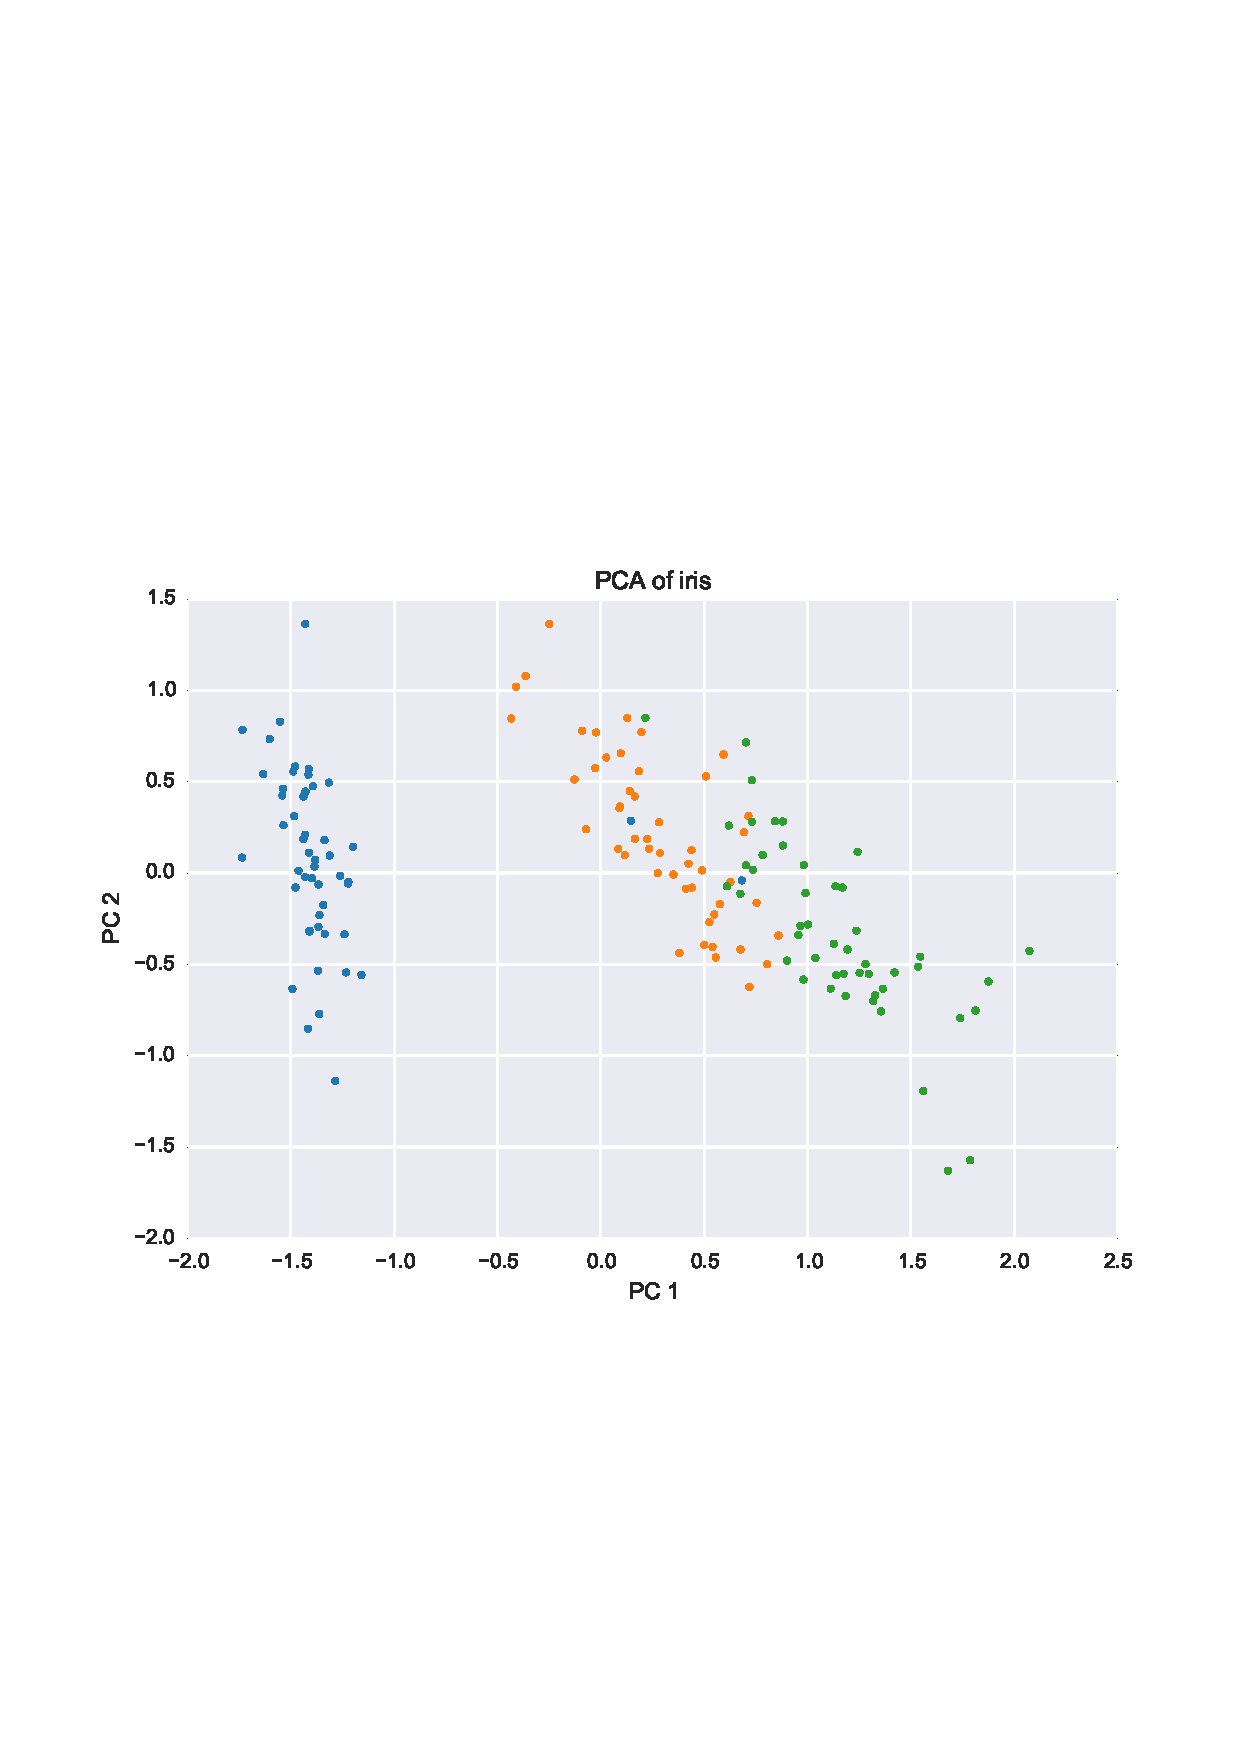
\includegraphics[scale=0.5]{Horn/img/iris_natural.png}
% \caption{Plot of the two first principal components (PC).}
% \label{fig:iris_natural}

% \end{figure}

% I chose $\sigma=\frac{1}{4}$ to reproduce the experiments in [3]. Only the first two PC are used here, which account for $95.8\%$ of the energy. The clustering results can be seen in Fig. \ref{fig:iris_2pc_cluster} and have an accuracy of 86\% computed with consistency index.


% \begin{figure}[hbtp]
% \centering
% 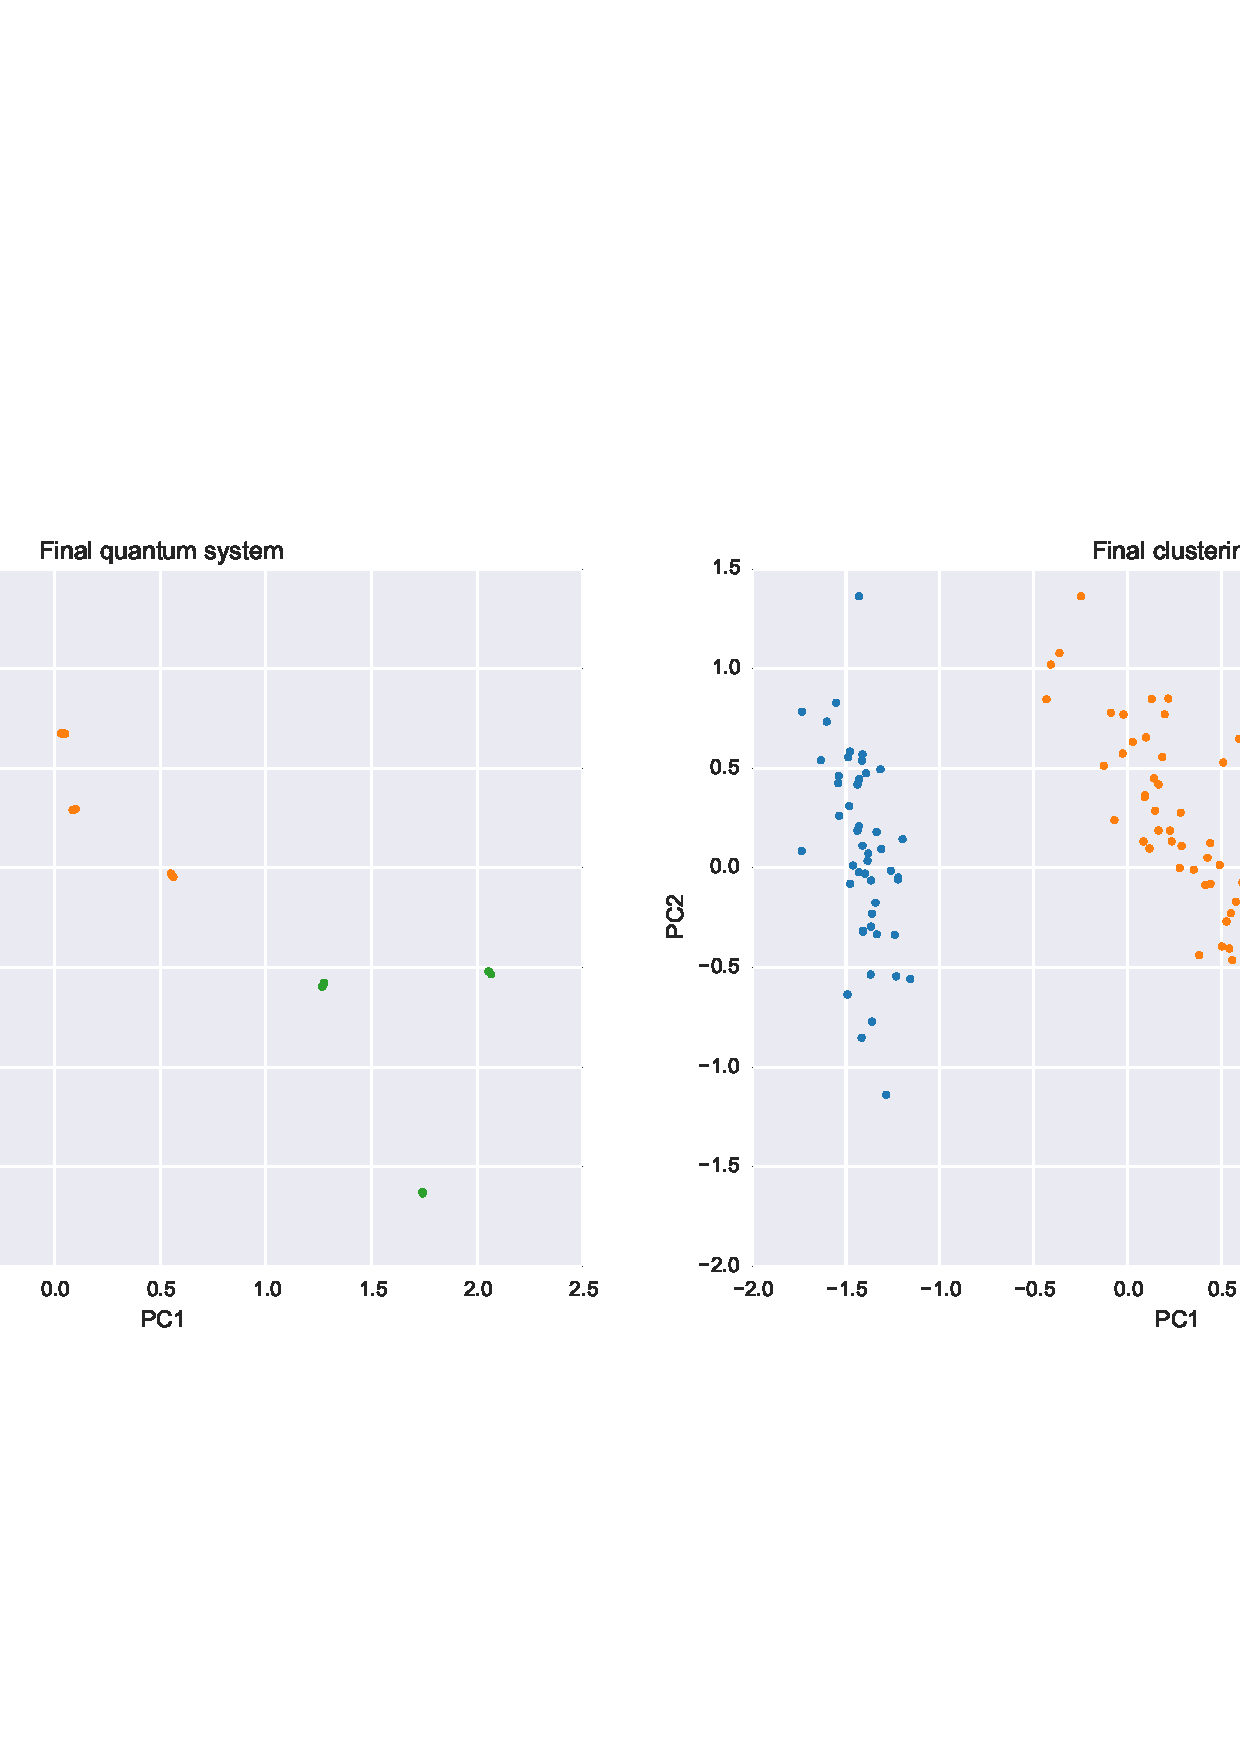
\includegraphics[width=\textwidth]{Horn/img/iris_2pc_cluster.png}
% \caption{Plots of the converged data data points and final clustering for 2 PC.}
% \label{fig:iris_2pc_cluster}

% \end{figure}

% For the sake of completeness, Fig. \ref{fig:iris_allpc_cluster} shows the clustering over all PCs. This solution has an accuracy of 82.67\% computed with consistency index.


% \begin{figure}[hbtp]
% \centering
% 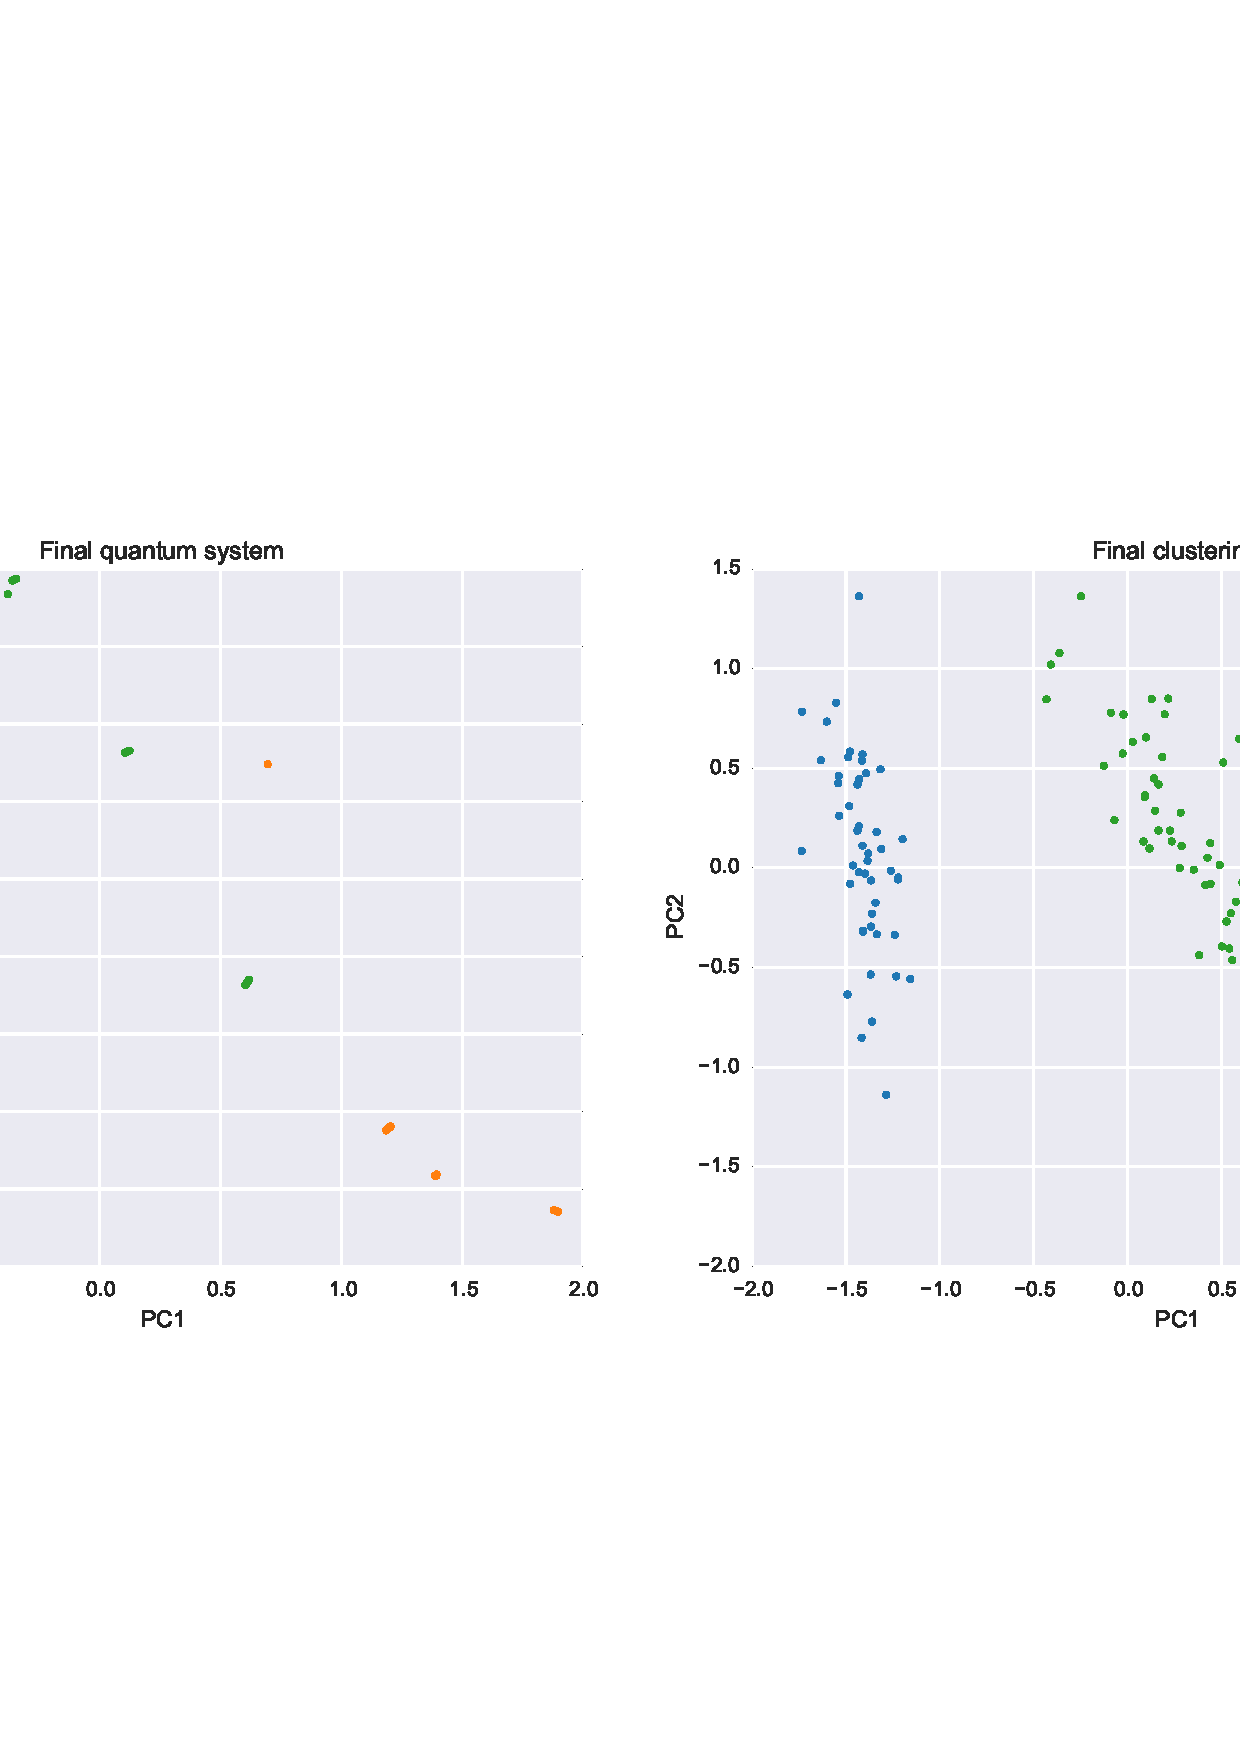
\includegraphics[width=\textwidth]{Horn/img/iris_allpc_cluster.png}
% \caption{Plots of the converged data data points and final clustering for all PC of Iris data.}
% \label{fig:iris_allpc_cluster}
% \end{figure}


% \subsection{Crab data}

% The crabs dataset has 200 samples and describes 5 morphological measurements on 50 crabs each of two colour forms and both sexes (total of 200 crabs), of the species Leptograpsus variegatus collected at Fremantle, Western Australia. After a preprocessing using PCA with covariance matrix and uncentred data, the dataset is represented in Fig. \ref{fig:crab_2pc_covar}.% #TODO add reference to dataset -->

% \begin{figure}[hbtp]
% \centering
% 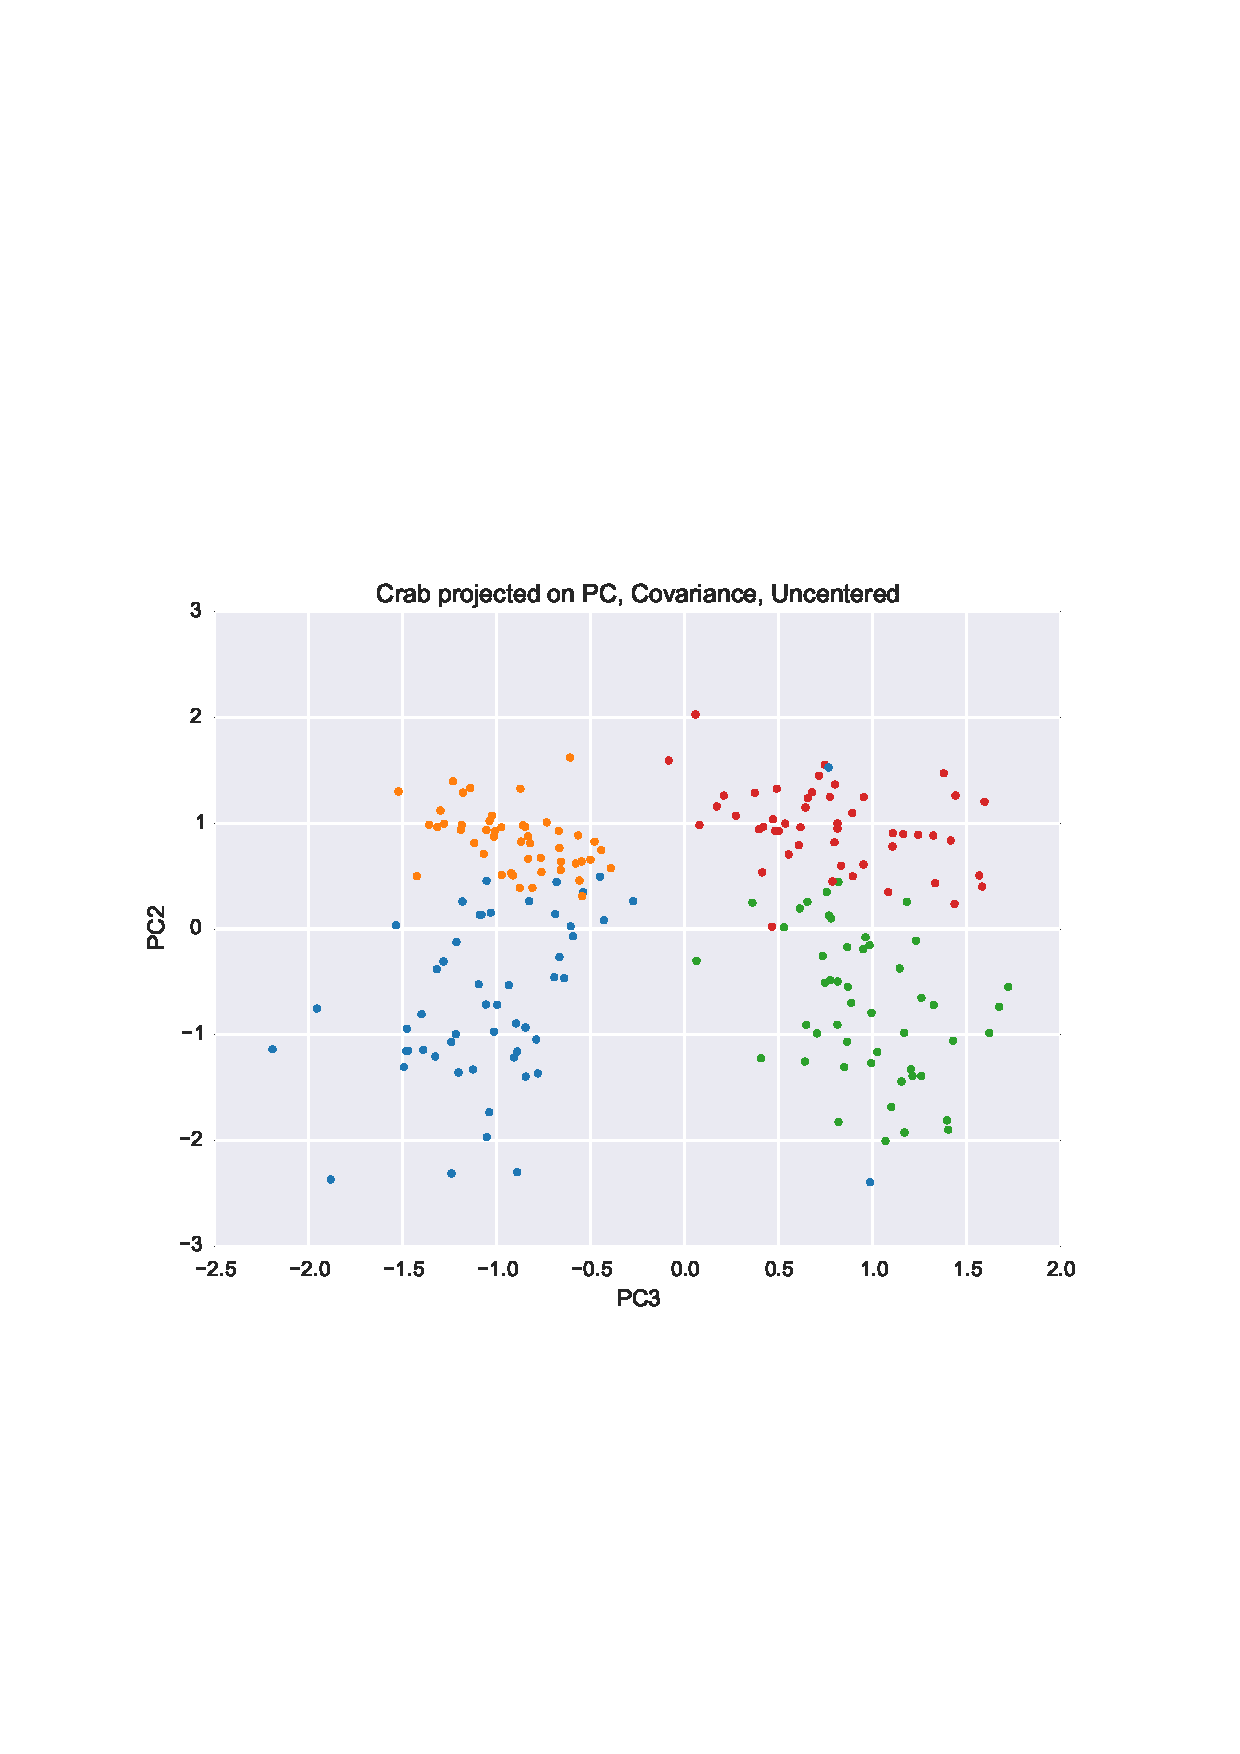
\includegraphics[scale=0.5]{Horn/img/crab_2pc_covar.png}
% \caption{Representation of the crab data projected over PC 2 and 3.}
% \label{fig:crab_2pc_covar}
% \end{figure}

% \begin{figure}[hbtp]
% \centering
% 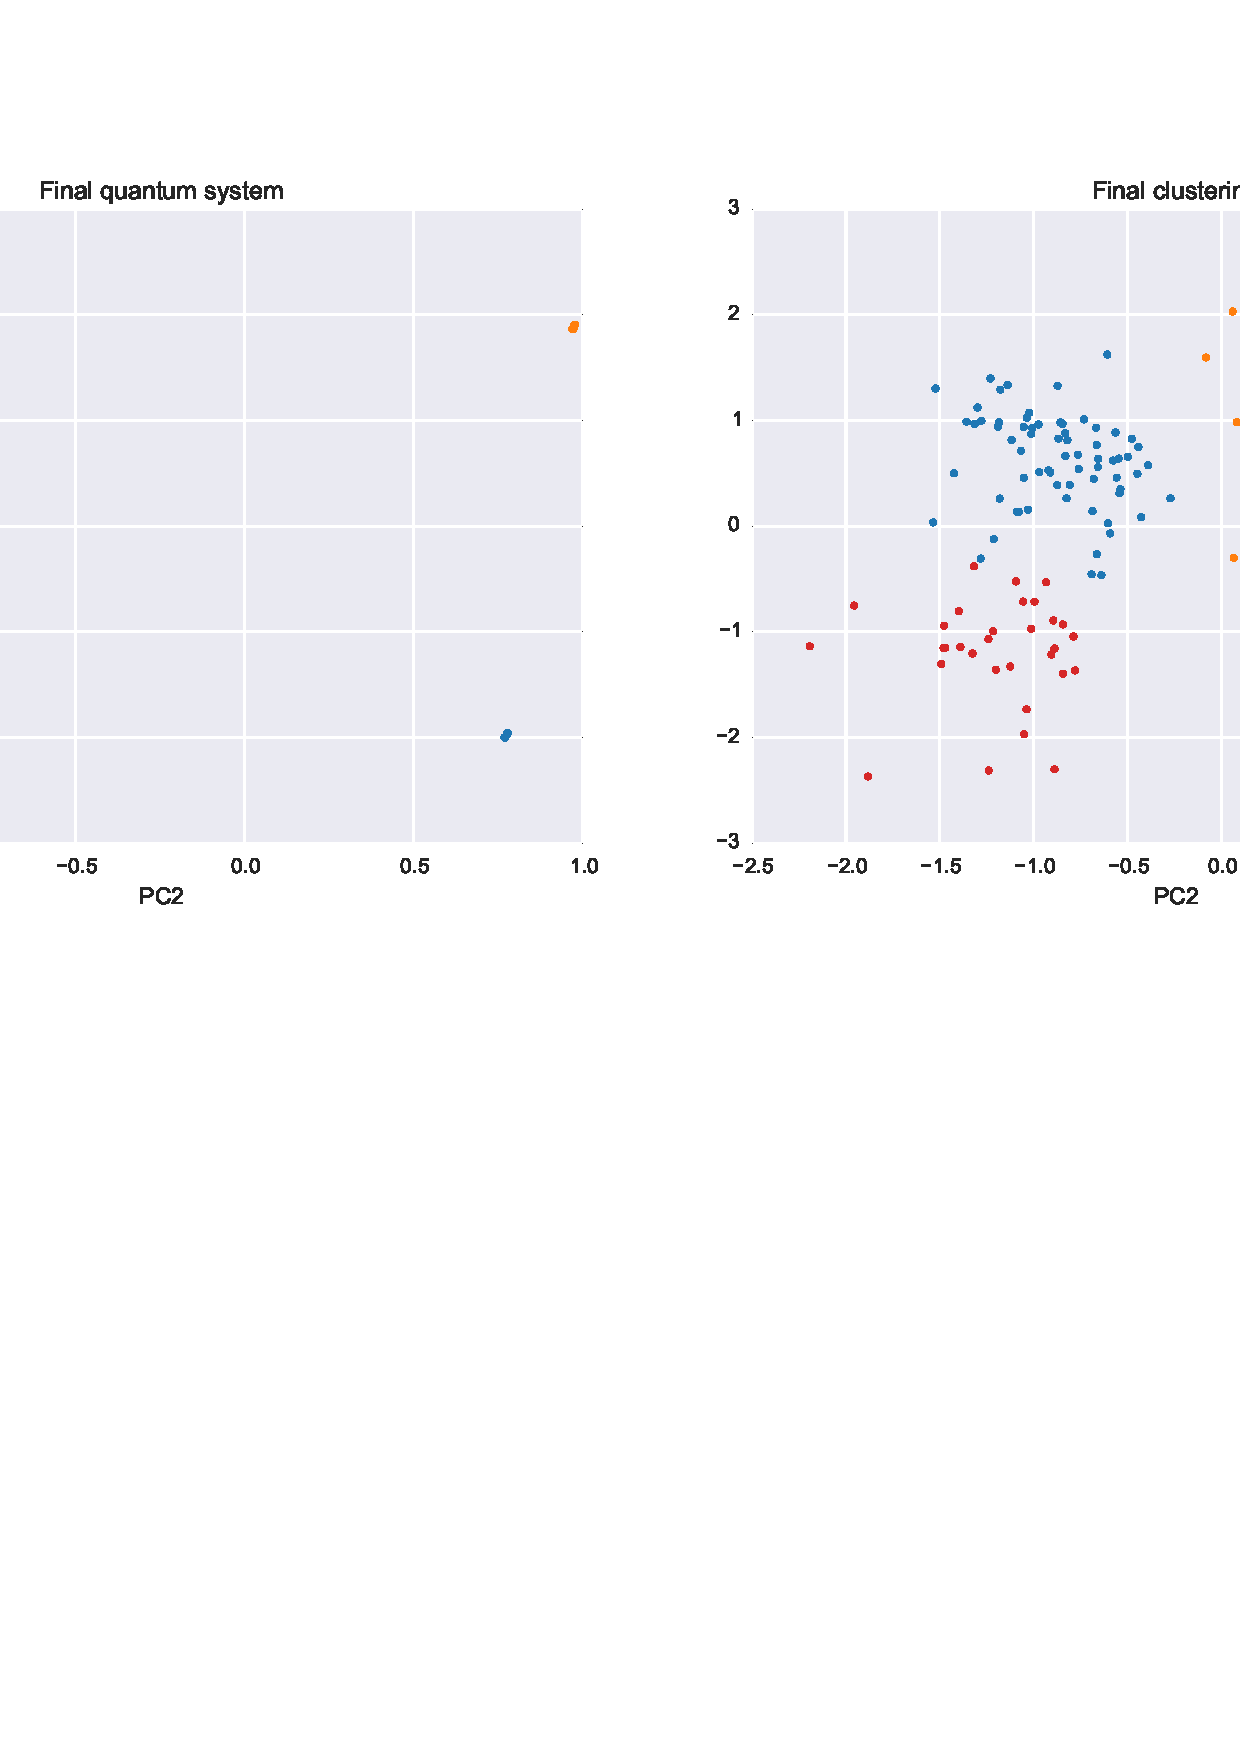
\includegraphics[width=\textwidth]{Horn/img/crab_2pc_covar_cluster.png}
% \caption{Representation of the crab data projected over PC 2 and 3.}
% \label{fig:crab_2pc_covar_cluster}
% \end{figure}

% \begin{figure}[hbtp]
% \centering
% 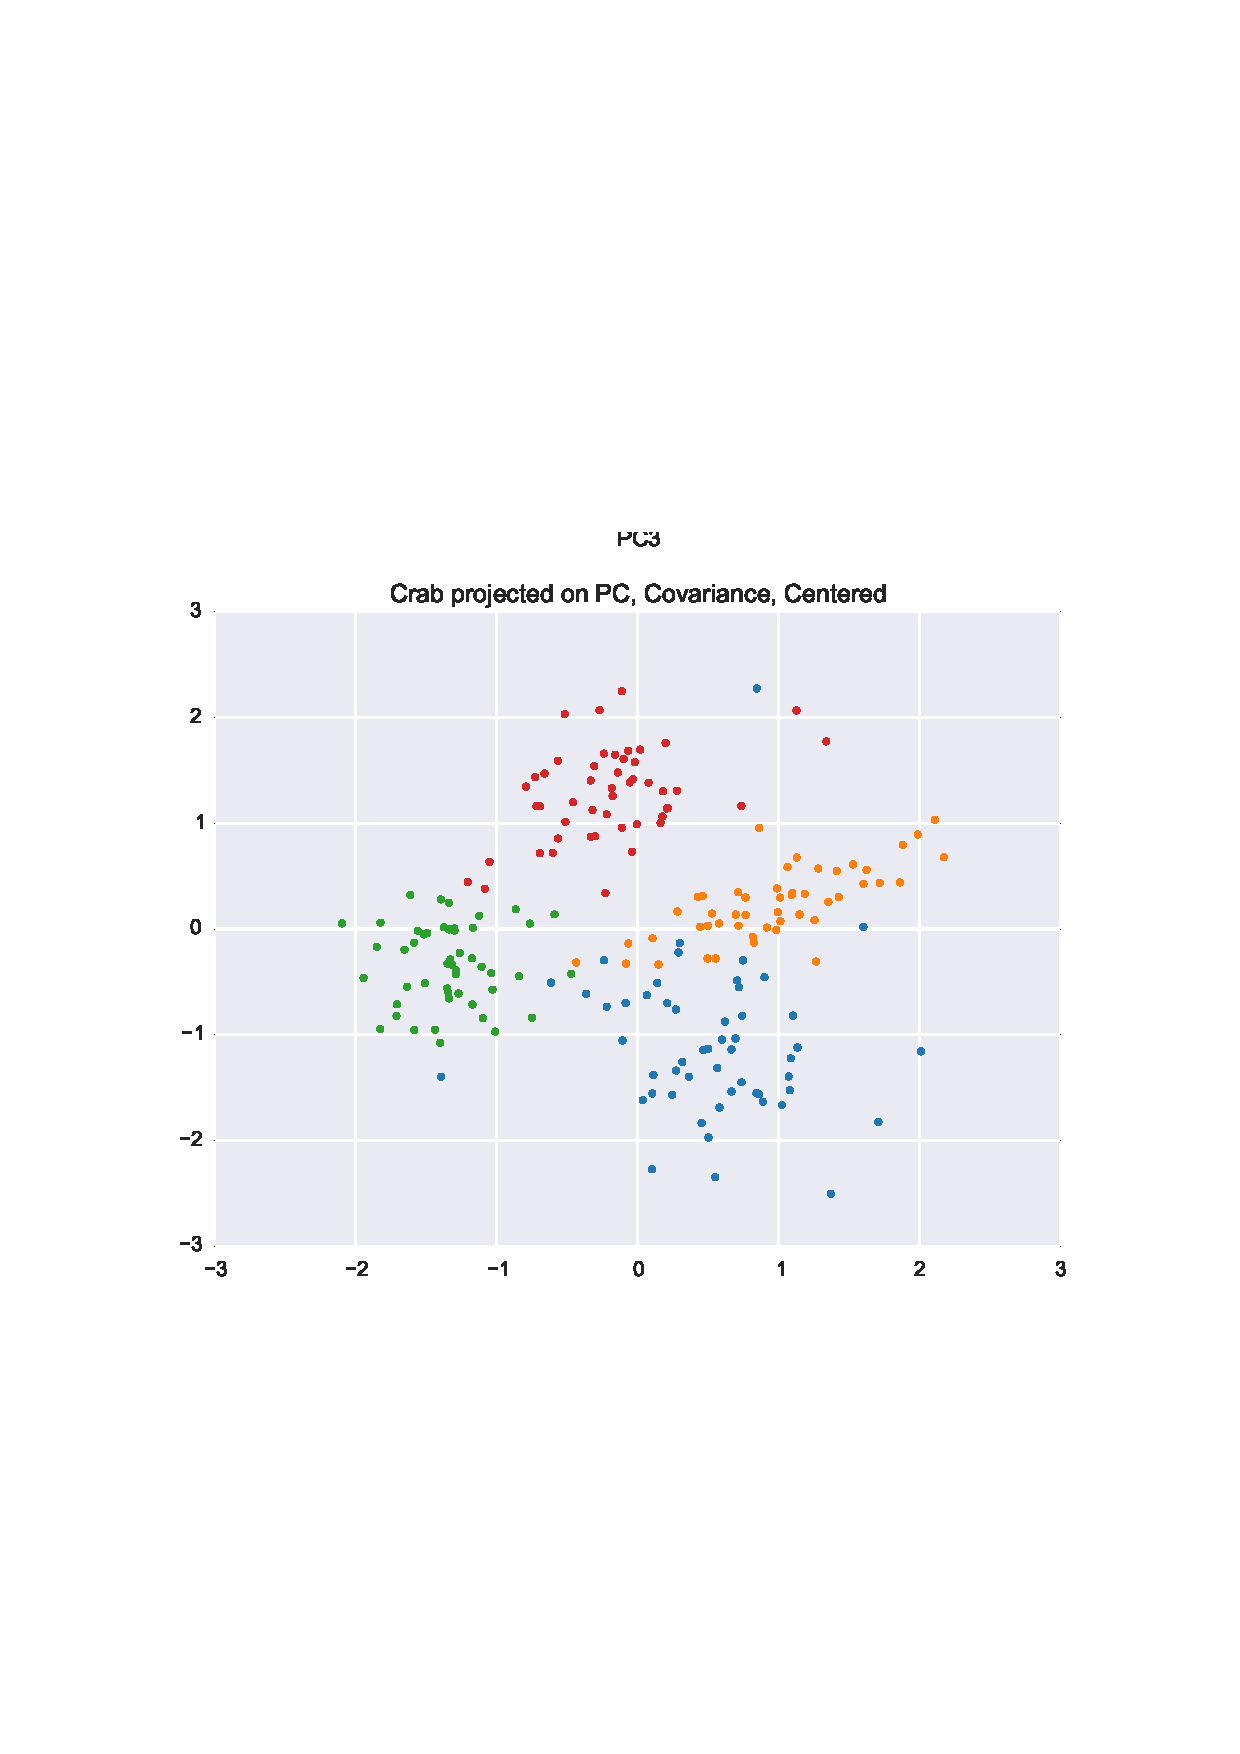
\includegraphics[scale=0.5]{Horn/img/crab_2pc_covar_centered.png}
% \caption{Representation of the crab data projected over PC 2 and 3.}
% \label{fig:crab_2pc_covar_centered}
% \end{figure}

% \begin{figure}[hbtp]
% \centering
% 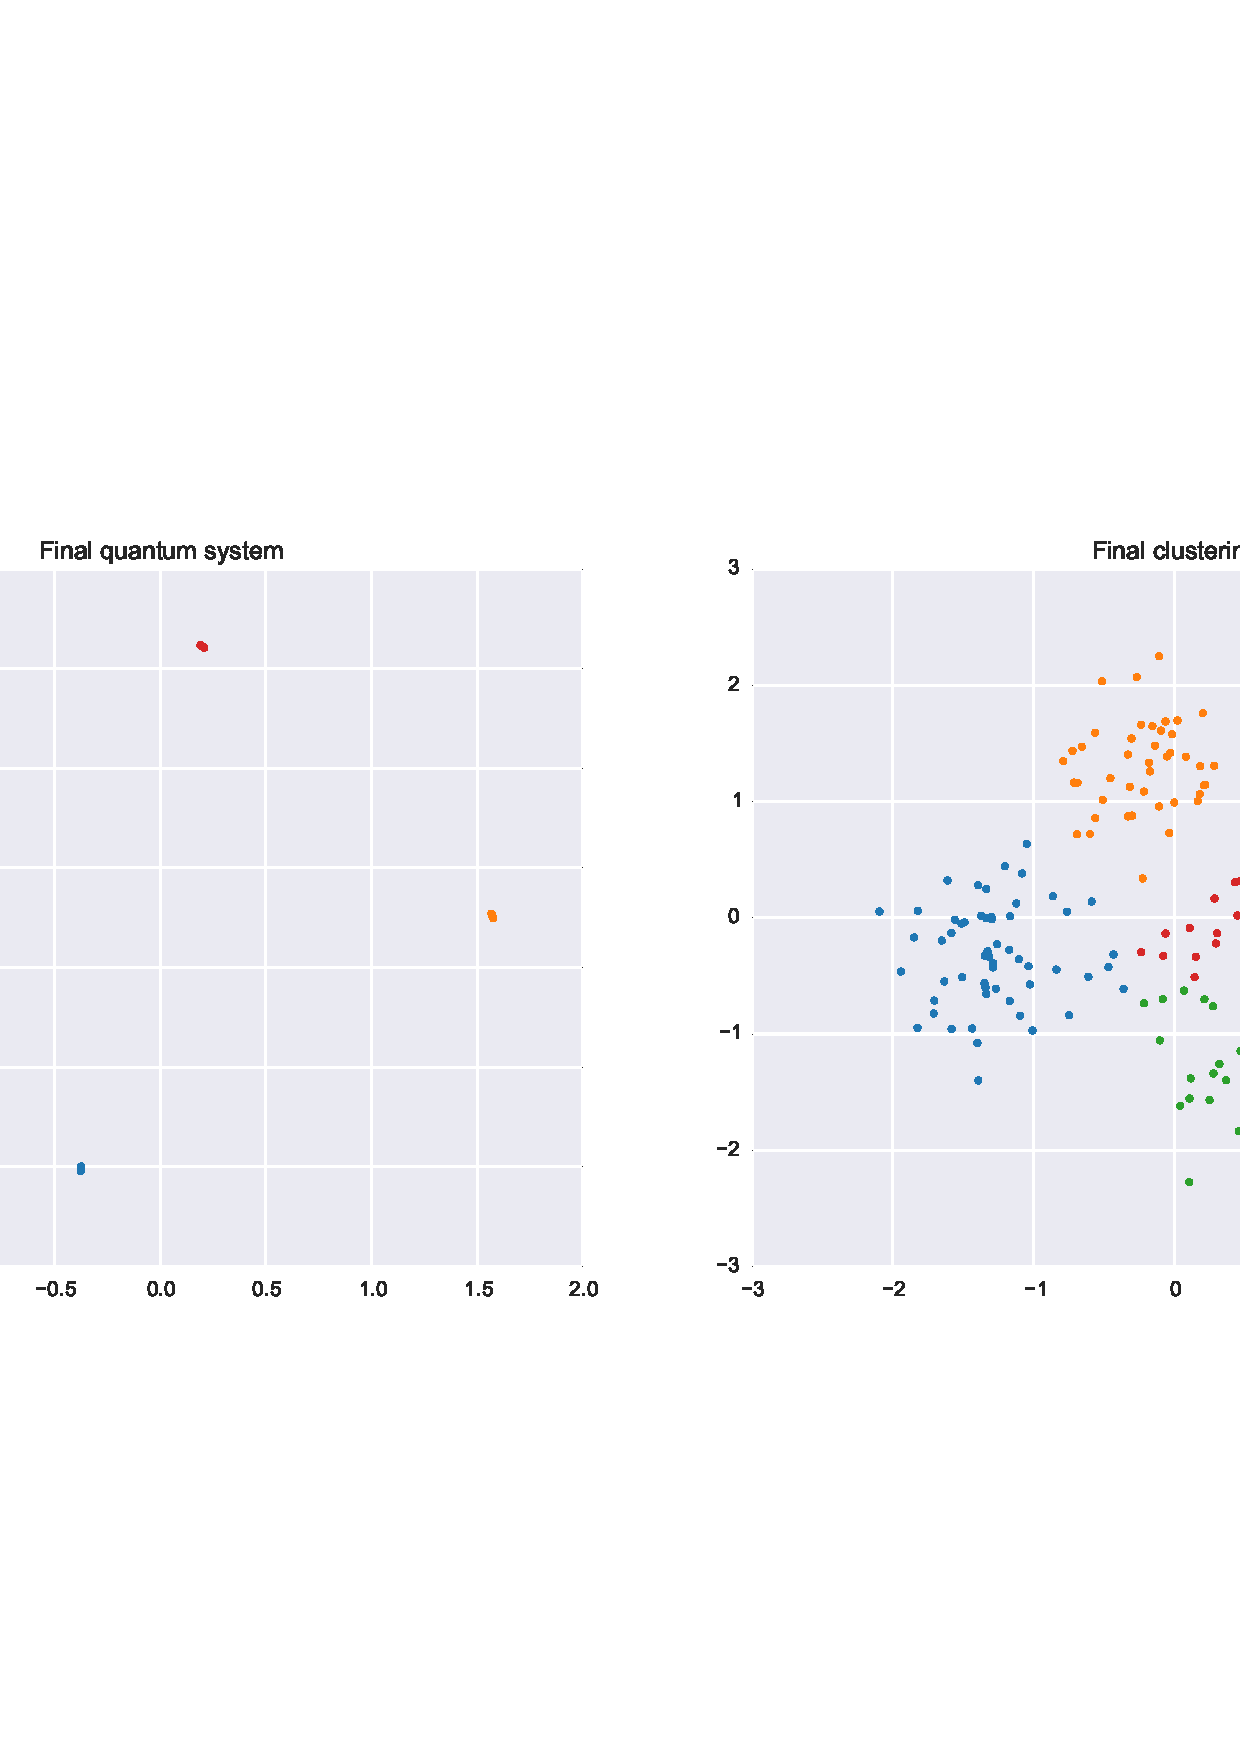
\includegraphics[width=\textwidth]{Horn/img/crab_2pc_covar_centered_cluster.png}
% \caption{Representation of the crab data projected over PC 2 and 3.}
% \label{fig:crab_2pc_covar_centered_cluster}
% \end{figure}


% Initial work aimed at reproducing results from [2], but lack of detail on the preprocessing used made it an harder task. Several preprocessings were used, namely whitening or not the data, centring it or not, using covariance versus correlation and different methods of computing the PCs through eigenvalue decomposition or Singular Value Decomposition (SVD). The closest representation to that of the [2] is the one if Fig. C1.


% %TODO finish crab

% Covariance uncentred consistency index = 0.815
% Covariance centred consistency index = 0.91

% all pc covariance uncentred consistency index = 0.63
% all dimensions original data consistency index = 0.34


\section{Discussion?}

%TODO
% in the Discussion or Conclusions chapter, include a reflection along the folloing lines
When a problem of clustering of big data is at hand, the user should reflect upon what the problem at hand really requires: speed or accuracy. The user should take into consideration the nature of the data and the requirements of the problem (concerning speed and accuracy) before proceeding to the execution of the analysis. The present body of work reflects a method of clustering over big data using a high accuracy, but also high cost, method. Other methods offer the opposite, low cost, low to average accuracy. 

\section{Future work}

Adaptation of the present implementation to OpenCL. This brings major benefits in respect to portability since OpenCL supports most devices. Moreover, OpenCL's performance is catching in on that of CUDA's and since it's programming model was based on CUDA, it should be straightforward for developers to make the switch.

Application of EAC to the MapReduce framework will further expand the possibilities of application of EAC.

Study the integration of other clustering algorithms within the the EAC toolchain.



\bibliographystyle{plain}
\bibliography{library}

\end{document}